\documentclass{article}

\usepackage{graphicx}
\usepackage{hyperref}
\usepackage{tikz}
\usepackage{float}
\usepackage{pgfplots}
\usepackage{cleveref}
\usepackage[toc,page]{appendix}
\usepackage{amsmath}


\author{Pintilie Andrei, Tabarcea Augustus}
\title{Clinical Brain Computer Interfaces}

\begin{document}
\maketitle

\section{Introduction}
\subsection{Motivation}

\section{Method}

\subsection{1D Convolutional}

As we saw in\cite{Deep_series} a very successful approach to time series is to use a \textit{Convolutional neural network}\cite{Convolutional_neural_network}.
We used a popular architecture\autoref{Conv1D_Arhitecture} to create a goal for our NeuroEvolution algorithms.

\subsection{NEAT}

Following the paper\cite{NEAT} we applied topological evolution of the artificial neural network used.
NEAT recommendation is to start with a small network and evolve from there, so we started with just the input and output layers.
The mutation is made by changing a property (connections,weights,bias) of a chosen node to mutate.
NEAT handles crossover this by keeping track of the origins of the nodes, with an identifying number (new, higher numbers are generated for each additional node).
Those derived from a common ancestor (that are homologous) are matched up for crossover, and connections are matched if the nodes they connect have common ancestry.
The probabilities for mutation and crossover are underlying properties of the package that we use, but they let us choose the probability for a change in the network as follows:
\begin{itemize}
  \item A node can either be disable,deleted or enabled,added.
In our case this probability is $\mathcal{P}(N_+)=0.2$ and a $\mathcal{P}(N_-)=0.2, $ where $N_+=\text{adding a new node}$ and $N_-=\text{removing a node}$.
  \item A node can either gain a new connection or lose it.
In this case we use $\mathcal{P}(C_+)=0.5$ and a $\mathcal{P}(C_-)=0.4, $ where $C_+=\text{adding a new connection}$ and $C_-=\text{removing a connection}$.
  \item A node can modify its weights.
We use for that a $\mathcal{P}(W_C)=0.8$ and a $\mathcal{P}(W_R)=0.1, $
where $W_C=\textrm{change the weight by adding or subtracting}\\ \textrm{with value from a gaussian distribution centered on 0 }$\\
and $W_R=\text{replacing the weight value}$.
\end{itemize}

\section{Experiment}

\section{Results}

\subsection{Interpretation}

\section{Conclusions}


\begin{appendices}

\begin{figure}[!ht]
  \centering
  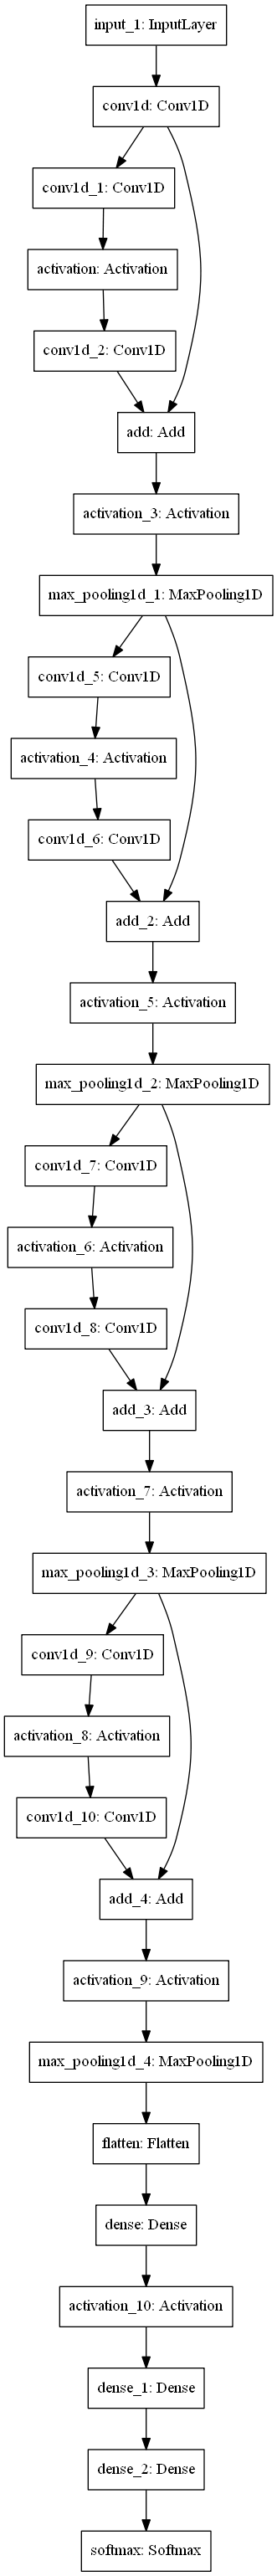
\includegraphics[width=\textwidth,height=\textheight,keepaspectratio]{model}
  \caption{Conv1D Arhitecture.}
  \label{Conv1D_Arhitecture}
\end{figure}

\end{appendices}

\begin{thebibliography}{9}
\bibliographystyle{plain}

\bibitem{Deep_series}
  Deep learning for time series classification by Hassan Ismail Fawaz, Germain Forestier,Jonathan Weber, Lhassane Idoumghar, Pierre-Alain Muller [2019]
  \url{https://arxiv.org/pdf/1809.04356.pdf}

\bibitem{Convolutional_neural_network}
  1D Convolutional Neural Networks and Applications by Serkan Kiranyaz, Onur Avci, Osama Abdeljaber, Turker Ince, Moncef Gabbouj, Daniel J. Inman [2019]
  \url{https://arxiv.org/ftp/arxiv/papers/1905/1905.03554.pdf}

\bibitem{NEAT}
  Efficient Reinforcement Learning through Evolving Neural Network Topologies by Kenneth O. Stanley and Risto Miikkulainen [2002]
  \url{http://nn.cs.utexas.edu/downloads/papers/stanley.gecco02_1.pdf}

\end{thebibliography}
\end{document}
